\newpage
\section{Un autre exemple}
\q{Dessiner les lignes de niveau de $h(x, y) = x^4 + y^4 - 4xy$}
\begin{dinglist}{111}
  \item On redéfinit \il{h} :
  \codeFromFileT{main.py}{section-08/qa.py}

  \item On redéfinit \il{nabla} qui doit maintenant retourner $\nabla h(x, y)$
  \codeFromFileT{main.py}{section-08/qb.py}

  \item On pense à changer \il{f} en \il{h} dans \il{points} et \il{ligne}.
  Puis on affiche :
  \codeFromFileT{main.py}{section-08/qc.py}
  Ce qui donne :
  \begin{center}
    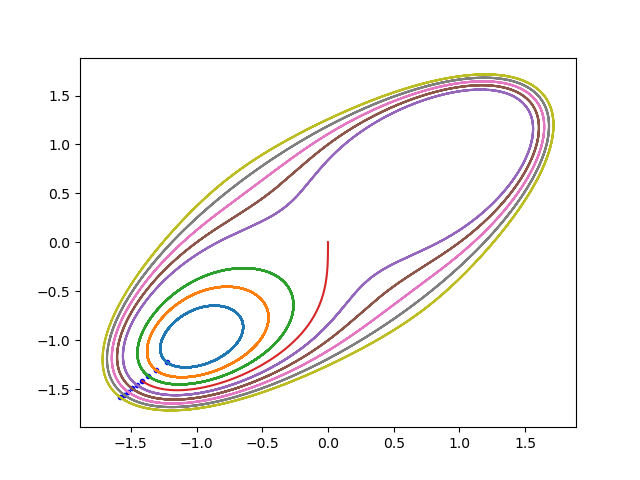
\includegraphics[scale=0.6]{section-08/qd.png}
  \end{center}

\end{dinglist}
